\documentclass[12pt, spanish]{article}
\usepackage[margin=1in]{geometry}
\usepackage[spanish]{babel}
\selectlanguage{spanish}
\usepackage[utf8]{inputenc}
\setlength{\parindent}{2cm}
\usepackage{hyperref}
\usepackage{graphicx}
\usepackage{float}

% Title Page
\title{Trabajo Práctico Final}
\author{Python Intermedio - UNLAR 2020}


\begin{document}
\maketitle

\section{Ejercicio}

Subir a la plataforma todo el código desarrollado.

El objetivo es desarollar una utilidad (simplificada) que simule el comportamiento
del comando "tree" de Linux. El resultado es mostrar algo así:

\begin{figure}[h]
	\centering
	\includegraphics[width=0.7\linewidth]{"1"}
	\label{fig:---3}
\end{figure}

Desarrollar esa utilidad será algo complejo para hacerlo en el tiempo que tenemos
por lo que vamos a simplificarlo. En primer lugar vamos a liberarnos de la tarea
de consultar el arbol de directorio del sistema operativo, y vamos a simularlo.

Luego vamos a crear la posibilidad de que el el usuario pueda elegir como presentar
el árbol, si es que lo hacemos al estilo de unix, como el que se mostró en la imagen
o lo hacemos en un formato ascii como el de la siguiente imagen:

\begin{figure}
	\centering
	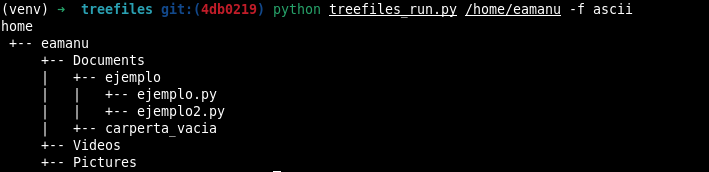
\includegraphics[width=0.7\linewidth]{2}
	\label{fig:2}
\end{figure}


Dentro del comprimido se encuentra  un archivo requirements.txt que es el que tiene
todas las depedencias necesarias para que el programa funcione. De ahi no deben modificar nada.

Dentro de la carpeta \textit{treefiles} se encuentran todos los archivos que necesitarán para que el programa funcione. Pero OJO hay errores y partes incompletas.

Leean atentamente el docstring del código porque puede dar algunas pistas, incluso hasta la solución.

Se debe hacer que el programa reciba parametros para ello van a utilizar argparse para facilitar esa tarea. 

EL programa debe pedir un "path" que es el que se va a listar (PERO RECUERDEN
AUNQUE SE PIDA EL PATH ESTO ESTÁ SIMULADO, ASÍ QUE NO IMPORTA QUÉ VALOR VA ACA) y 
otro parámetro que me indique el formato.

Por último hacer al menos 3 test unitarios para las funciones

Entonces las tareas son:

\begin{itemize}
	\item crear la función get\_simulate\_folder() que me devuelva un formato conocido dependiendo si quiero imprimir en formato unix o ascii, y que le guste a la biblioteca Ver docstring.
	\item Corregir los errores.
    \item Implementar lo que haga falta
    \item Hacer que la utilidad reciba los parametros: folder y format
    \item Hacer test unitarios.
\end{itemize}


\end{document}          
